\section{Introduction Historique}

\begin{frame}
    \frametitle{Contexte scientifique }
    \framesubtitle{Premiers modèles}

    Craig Reynolds (1987) : Premier modèle de mouvement de foule : les boids

    \begin{itemize}
        \item	<2->	Représentation de nuées d’oiseaux
        \item	<3->	Règles très simples
        \item   <4->      Vitesses et trajectoires des agents liées aux voisins proches

              \visible<5->{
                  \begin{figure}
                      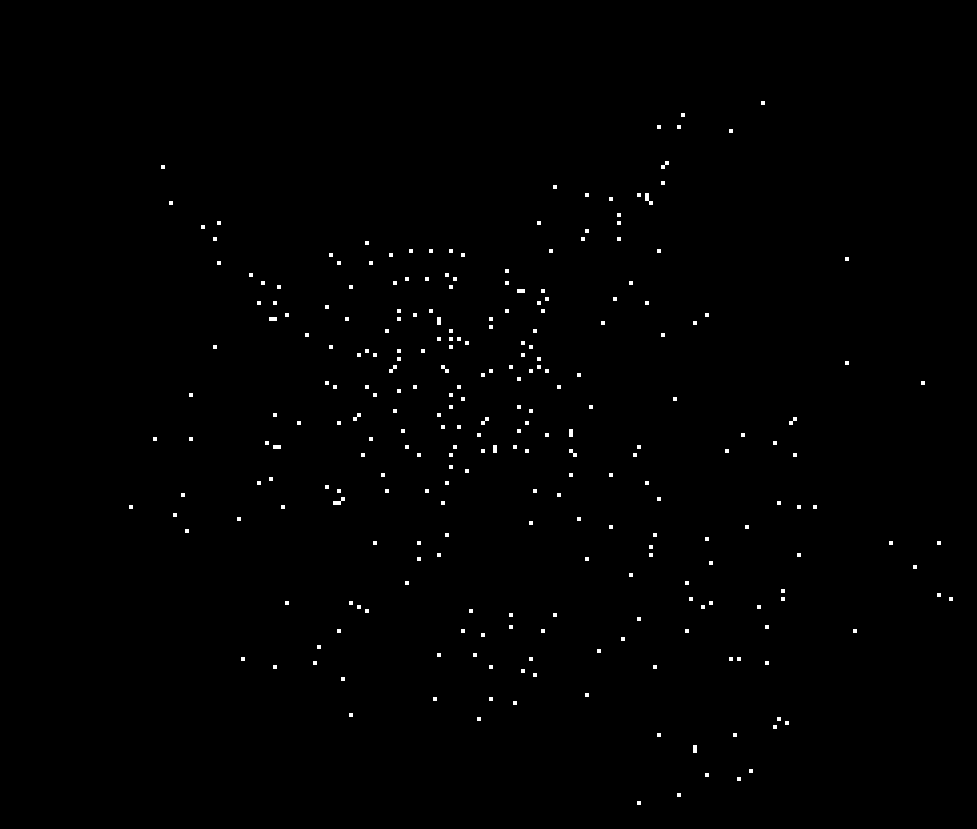
\includegraphics[width=0.5\linewidth]{figures/Fig01}
                  \end{figure}
              }

    \end{itemize}

\end{frame}


\begin{frame}
    \frametitle{Introduction historique}
    \framesubtitle{Premiers modèles}

    Dirk Helbing et Péter Molnar (1998) : Le concept de "forces sociales"

    \begin{itemize}
        \item	<2->	Force d’attraction sociale : les trajectoires peuvent être influencées

        \item	<3->	Force de répulsion : les contacts physiques sont évités
    \end{itemize}
    \bigskip
    \onslide<4-> Julien Pettre et Wouter Van Toll (2021) : Evitement de collision

    \begin{itemize}
        \item <5-> Les trajectoires sont adoucies et plus réalistes en fonction des obstacles
    \end{itemize}

\end{frame}


\begin{frame}
    \frametitle{Introduction historique}
    \framesubtitle{Modèles plus réalistes}

    \visible<1->{
        \begin{figure}
            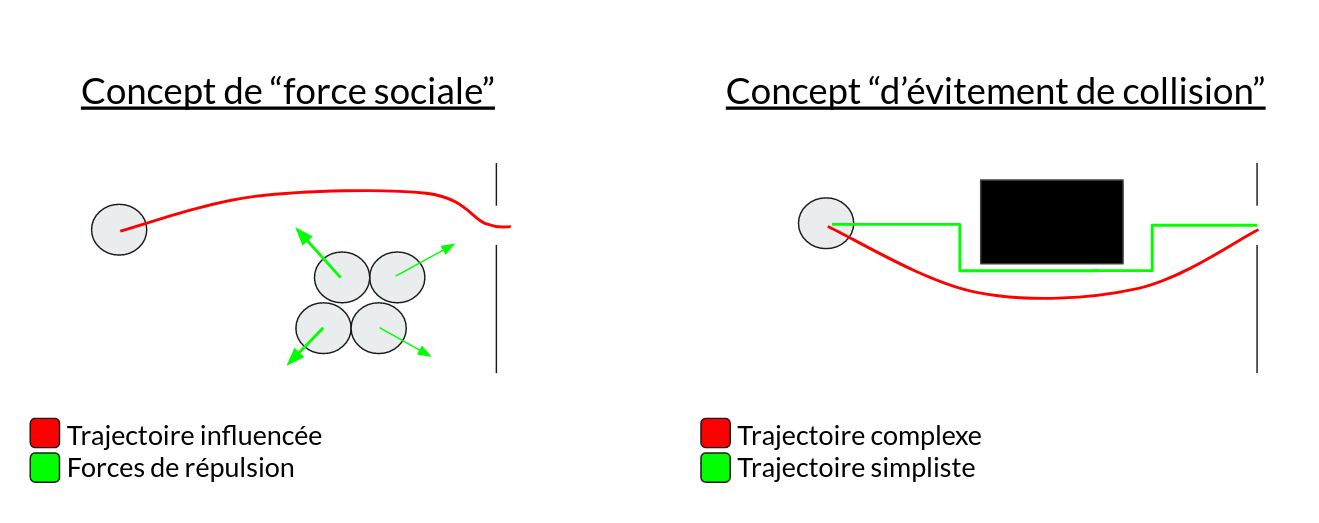
\includegraphics[width=1\linewidth]{figures/Fig02}
        \end{figure}
    }

\end{frame}
